
\FloatBarrier
\section{Workbench Architecture}
\label{sec:workbench-architecture}

\begin{figure}[htb]
\centering
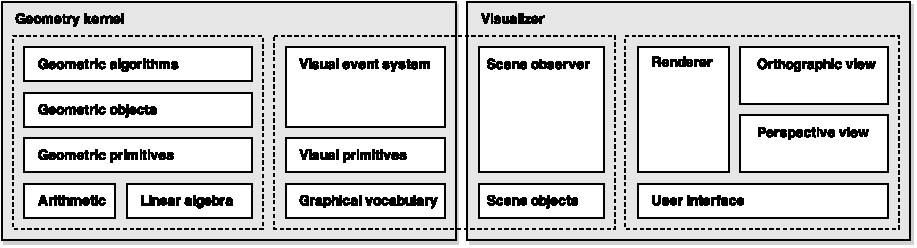
\includegraphics[width=\textwidth]{figures/components-uml-4} 
\caption{An abstract overview of the workbench architecture.}
\label{fig:components} 
\end{figure}

The workbench comprises two major components: a geometric algorithm library and
a geometric algorithm visualizer. The \emph{geometry library} implements
geometric algorithms. It defines types for arithmetic, linear algebra, and
geometric primitives (e.g. points, line segments, and triangles). These are
building blocks with which it defines more complex geometric objects (e.g.
polygons and polytopes). All of these may be used to implement geometric
algorithms. The \emph{visualizer} displays the execution of geometric
algorithms. It is structured using the model-view-controller (MVC) design
pattern. In particular, it maintains a visual model, several views of the visual
model, and a user interface that functions as the controller. In this section,
we are concerned with explaining how the kernel and visualizer work together to
produce algorithm visualizations.

\FloatBarrier
\subsection{The Geometry Library}

The \emph{arithmetic} and \emph{linear algebra} components are orthogonal to our
discussion of visualization. The \emph{graphical vocabulary} component is
necessary to define briefly but is straightforward to understand and depends
only on fundamental language types. In particular, it consists of types to
specify color, transparency, and a lighting model.

\emph{Geometric primitives} are geometric objects of constant size. We are
concerned with three: points, line segments, and triangles\footnote{Other
primitives include lines and rays but these are not directly supported by the
visual interface.}. Points are the basic unit of visualization. They are
equipped with unique identifiers (UIDs), assigned by registering with the visual
model. Line segments and triangles are combinatorial groupings of two and three
points, respectively. Thus, they are implicitly equipped with unique identifiers
given by the combinatorial grouping of their points' UIDs.

\emph{Visual primitives} are types that define the subset of graphical
vocabulary applicable to a corresponding geometric primitive. For
example, a visual point type might specify that points may be assigned a color
and rendered as either a circular or square sprite; a visual segment type might
also specify a color attribute but have no notion of a sprite shape.

The \emph{visual event system} defines the notion of observable geometry.
\emph{Observable geometry} objects notify their observers of changes in their
visual state by emitting signals. \emph{Geometry observers} handle these
notifications by implementing a corresponding slot. All higher level geometric
types that wish to be rendered by the visualizer must implement the observable
geometry interface. If a geometric object is composed of other observable
geometry objects, then it must also implement the geometry observer interface
and subscribe to those other objects.

Many geometric types will be composed of other observable geometry objects, so
we define an abstract base class that is both observable and capable of
observing other objects. By default, this base class forwards any visual events
it receives from the objects it observes onward to its own subscribers. In this
way, visual events are passed through a chain of event handlers, eventually
arriving at the scene observer in the visualizer.

\begin{figure}[htb]
\centering
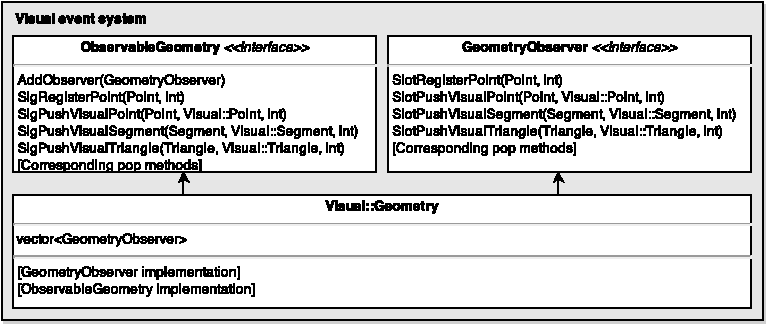
\includegraphics[width=\textwidth]{figures/visual-uml-6} 
\caption{The visual event system embedded in the geometry kernel.}
\label{fig:visual} 
\end{figure} 

\FloatBarrier
\subsection{The Visualizer}

\emph{Scene objects} are wrappers around geometric objects that implement an
interface required by the scene observer (e.g. being selectable or having a
name). Scene objects observe the geometric object they wrap, and may be observed
by the scene observer.

The \emph{scene observer} is the ultimate destination for all visual events
produced by geometric objects. It maintains three maps that pair unique
geometric primitives with a stack of visual primitives, the top of which defines
the current visual state. The scene observer is responsible for translating the
graphical vocabulary defined in the kernel into OpenGL buffer objects. The scene
observer lives inside of its own thread, and each of the visual events emitted
from an observable object may be given an integer value that will pause this
thread for a corresponding number of milliseconds.

The \emph{renderer} is responsible for managing OpenGL data and state.The
\emph{orthographic view} provides a top-down orthographic projection of the
scene. The user may pan around the plane and zoom in/zoom out. The
\emph{perspective view} provides a perspective projection of the scene. The user
may arbitrarily orient the camera and travel forward and backward along the view
direction.
